\section{Combined Effects and Further Predictions}

Having derived separate time dilation factors for motion through æther and gravitational æther flow, we now consider both effects simultaneously.

\subsection*{Combined Motion and Gravitational Field}

Let a vortex-clock move with velocity $\vec{u}$ in a region where the æther is flowing with velocity $\vec{v}_g$. The effective relative velocity with respect to the local æther flow is:
\[
\vec{v}_\text{rel} = \vec{u} - \vec{v}_g.
\]
The observed time dilation is then:
\[
\frac{d\tau}{dt} = \sqrt{1 - \frac{|\vec{v}_\text{rel}|^2}{c^2}}. \tag{5}
\]
This formulation smoothly incorporates both special and general relativistic effects into a single expression.

\subsection*{Example: Circular Orbit Time Dilation}

Consider a clock orbiting a mass $M$ at radius $r$. The tangential velocity of the orbit is:
\[
v_\text{orb} = \sqrt{\frac{GM}{r}}, \quad v_g(r) = \sqrt{\frac{2GM}{r}}.
\]
Since the orbital velocity is perpendicular to the radial æther inflow, the relative speed is:
\[
v_\text{rel} = \sqrt{v_\text{orb}^2 + v_g^2} = \sqrt{\frac{3GM}{r}}.
\]

\begin{figure}[htbp]
    \centering
    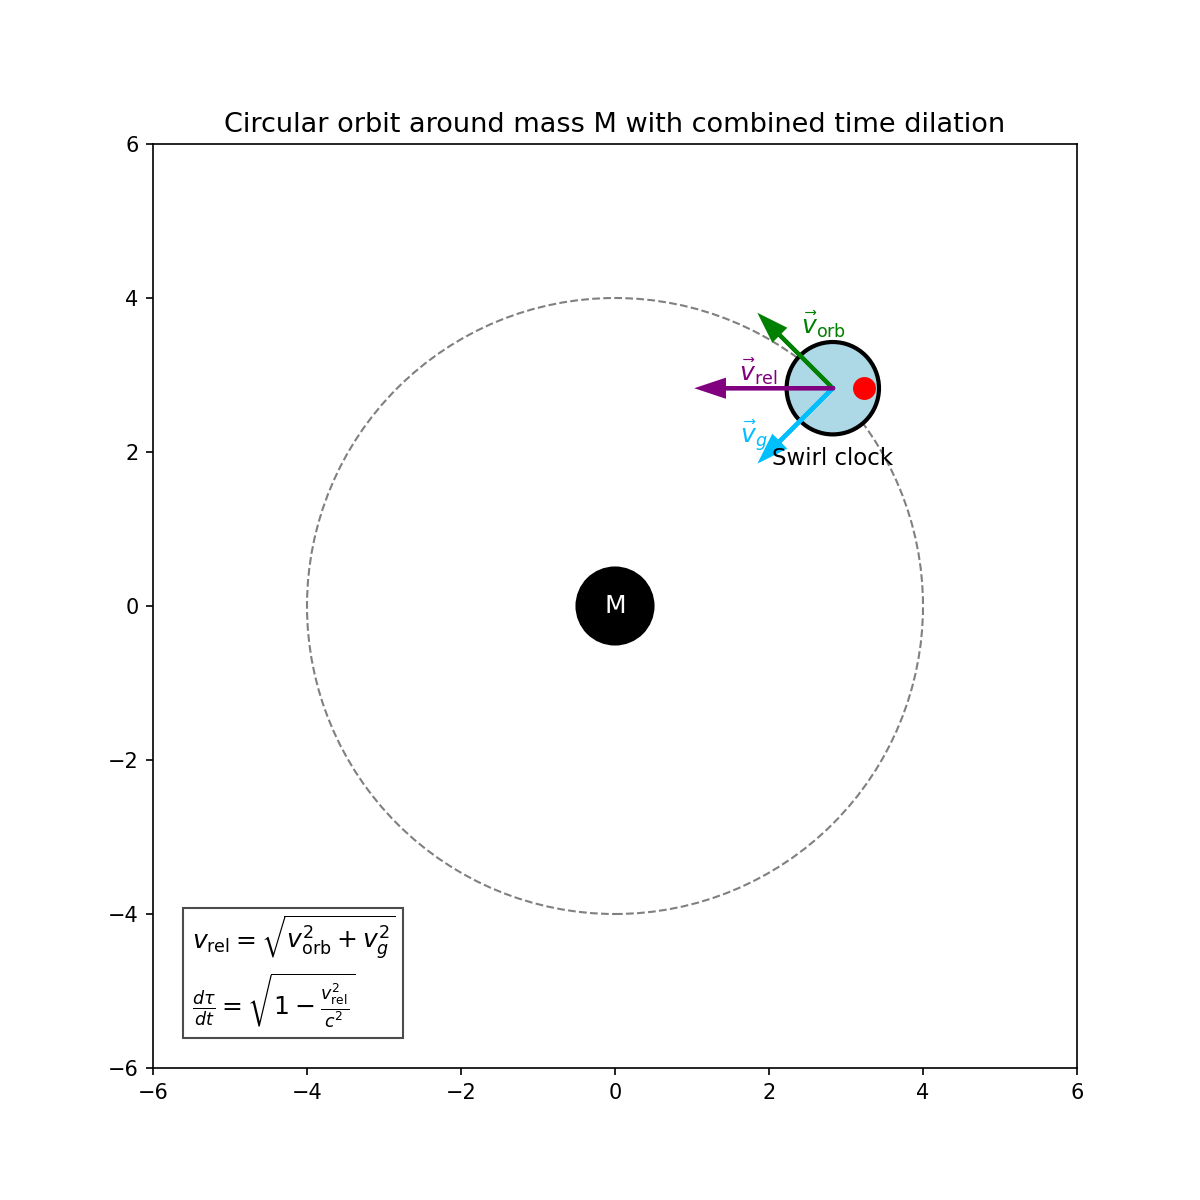
\includegraphics[width=0.85\textwidth]{images/08-BaanRondMassa}
    \caption{A vortex in a circular orbit experiences combined time dilation due to orbital and æther flow. The clock experiences both orbital velocity~$\vec{v}_{\mathrm{orb}}$ and æther inflow~$\vec{v}_g$, which together result in a combined relative velocity~$\vec{v}_{\mathrm{rel}}$.}
    \label{fig:BaanRondMassa}
\end{figure}

Thus, the time dilation becomes:
\[
\frac{d\tau}{dt} = \sqrt{1 - \frac{3GM}{rc^2}}. \tag{6}
\]
This matches the exact result from Schwarzschild geometry for circular orbits.

\begin{figure}[htbp]
    \centering
    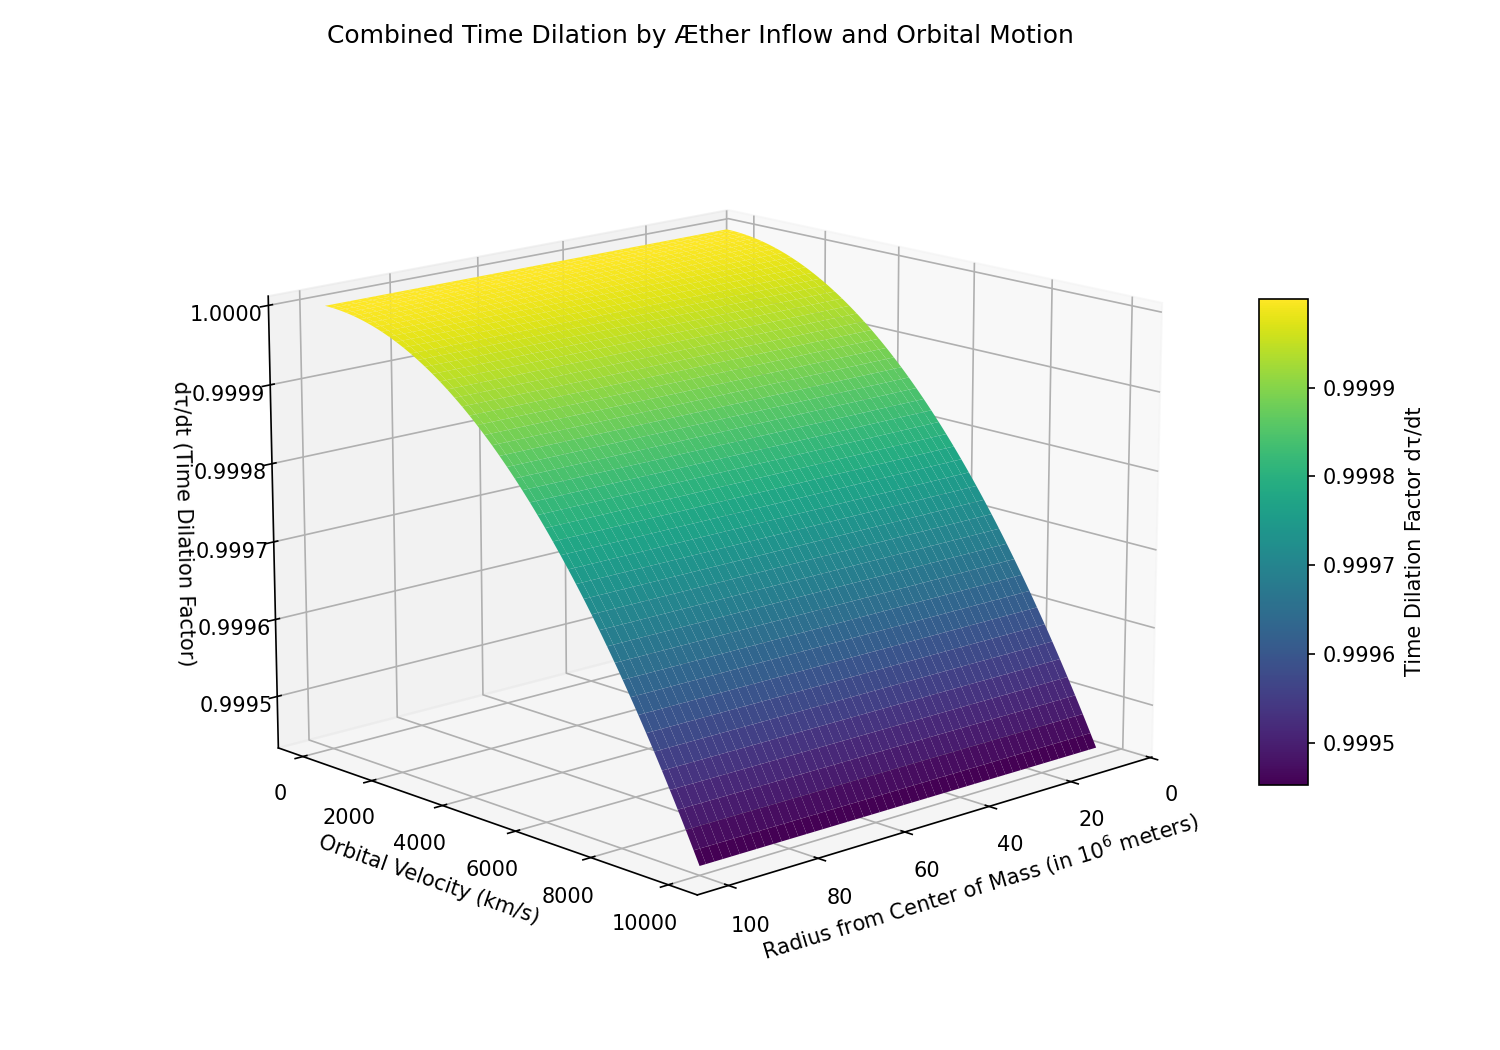
\includegraphics[width=0.85\textwidth]{images/09-CombinedTimeDilationSurface}
    \caption{Visual representation of the time dilation factor \( \frac{d\tau}{dt} \) as a function of both the orbital velocity \( v_\text{orb} \) and the gravitational æther inflow velocity \( v_g \). The surface shows how both contributions — inertial and gravitationally derived æther flow — together result in a total slowing down of the clock. The hyperbolic curvature of the surface reflects the combined Lorentz and Schwarzschild dilation as described in equations (5) and (6).}
    \label{fig:TimeDialationCombined}
\end{figure}

\subsection*{Implications Near a Horizon}

As $r \to r_s = 2GM/c^2$, the inflow speed $v_g(r)$ approaches $c$, and any static observer's clock slows to zero. The æther flow fully suppresses local vortex rotation, providing a natural mechanism for the \("\)freezing of time\("\) at the event horizon.

\begin{figure}[htbp]
    \centering
    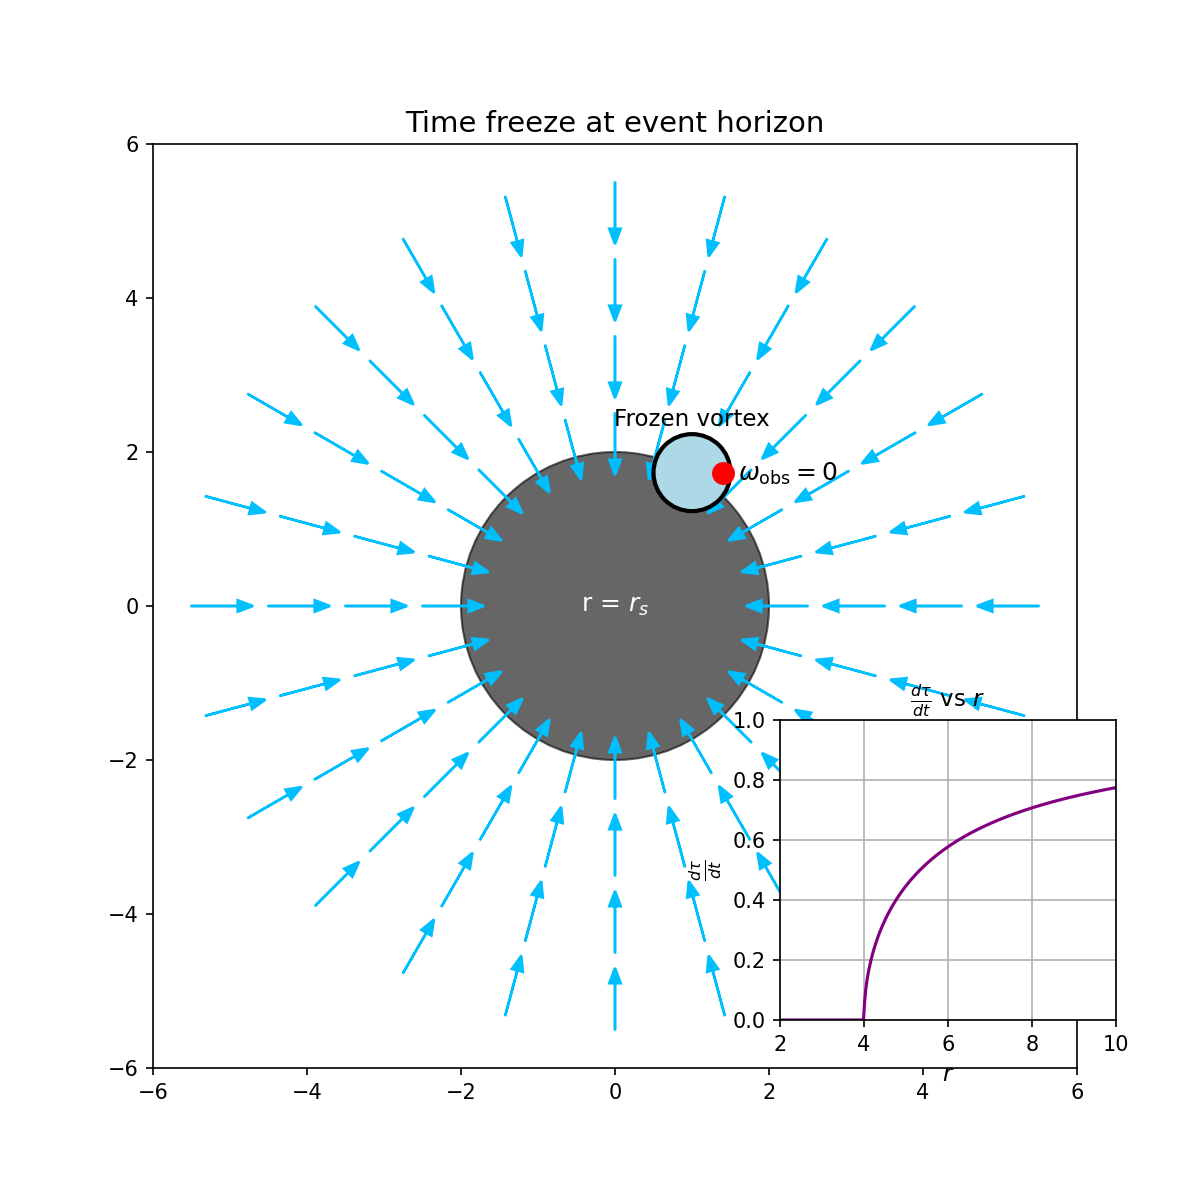
\includegraphics[width=0.85\textwidth]{images/10-HorizonTijdsbevriezing}
    \caption{Æther flow accelerates towards $r_s$, where the observed clock rotation becomes zero. Freezing of time at the event horizon $r = r_s$: the Æther flow approaches~$c$, causing $\omega_{\mathrm{obs}} \to 0$. On the right, the corresponding decrease in $\frac{d\tau}{dt}$ as a function of distance is shown.}
    \label{fig:HorizonTijdsbevriezing}
\end{figure}


\subsection*{Quantum and Cosmic-Scale Consistency}

This vortex-æther framework naturally explains relativistic phenomena consistently across scales—from quantum to cosmic. For instance, at quantum scales, the observed lifetime dilation of rapidly moving muons directly results from reduced internal vortex rotation frequency in relativistic æther flows. At cosmic scales, near black hole horizons, vortex rotation essentially freezes due to æther inflow approaching ccc, providing a concrete physical mechanism for horizon phenomena. Such scale invariance underscores the comprehensive explanatory power of the æther model.

\subsection*{Unified Interpretation}

\begin{figure}[htbp]
    \centering
    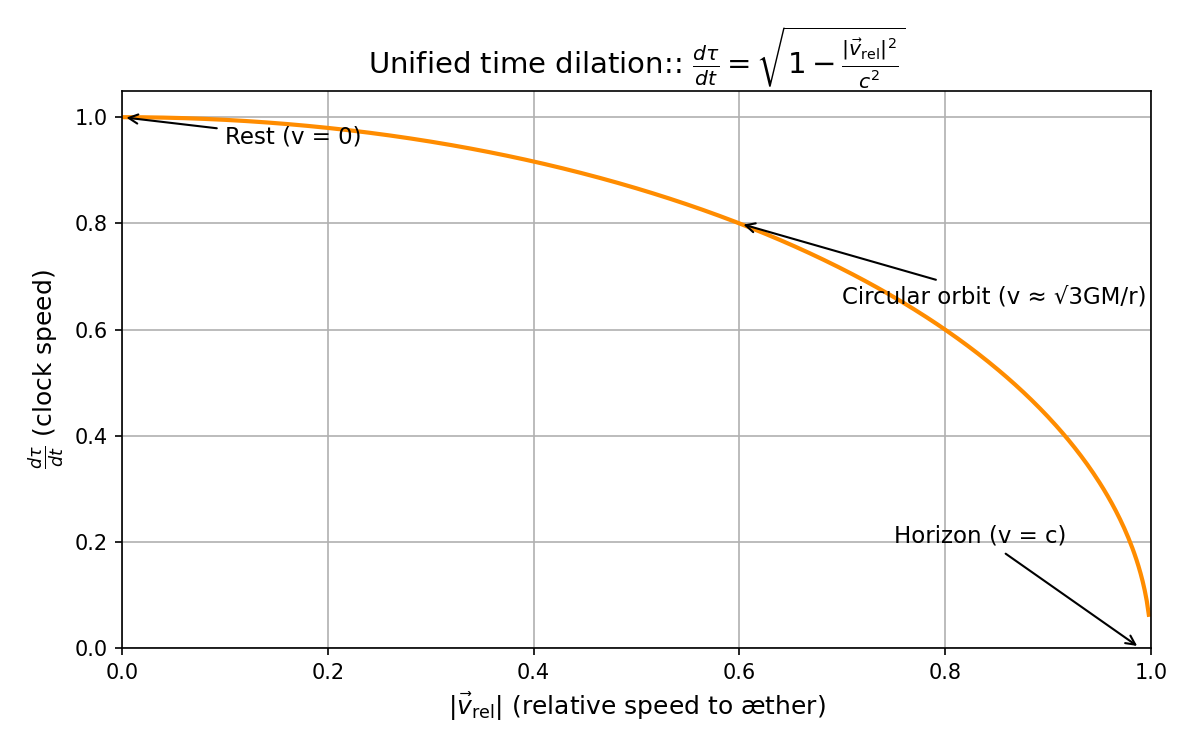
\includegraphics[width=0.85\textwidth]{images/11-TijdsvertragingRelatieveBeweging}
    \caption{Universal time dilation formula in the Vortex Æther Model. The clock rate decreases with increasing relative velocity~$|\vec{v}_{\mathrm{rel}}|$ with respect to the æther. At $|\vec{v}_{\mathrm{rel}}| = c$ time stops.}
    \label{fig:TijdsvertragingRelatieveBeweging}
\end{figure}

This æther model allows all relativistic time dilation effects to be viewed as consequences of one principle:
\[
\text{Clock rate reduction} \;\propto\; \text{relative motion through æther}.
\]
Whether this relative motion arises from inertial velocity or from ætheric inflow due to nearby mass, the observable consequence is the same. Therefore, we conclude:
\[
\boxed{\frac{d\tau}{dt} = \sqrt{1 - \frac{|\vec{u} - \vec{v}_g|^2}{c^2}}}
\]
as the general time dilation formula for the Vortex Æther Model.
For possible experimental deviations of these time dilation formulas from general relativity, see Appendix-B~\ref{appendix:DeviatingPredictions}.